\documentclass[11pt]{article}
\usepackage{colacl}
\usepackage{graphicx}
\usepackage[T1]{fontenc}
\usepackage[utf8]{inputenc}
\usepackage{amsmath}
\graphicspath{{img/}}
\DeclareUnicodeCharacter{F8FF}{$\diamond$}
\sloppy

\title{COMP30027 Assignment 2: Report}
\author
{Anonymous}



\begin{document}
\maketitle

\section{Introduction}\label{sec:intro}
% Introduction: a short description of the problem and data set

Sentiment analysis is a field of natural language processing focusing on the classification of text by its perceived sentiment.
It speeds up measuring the opinions of groups of people and can be applied in many fields such as marketing, politics or sociology.
My goal is to develop and train several reliable {T}witter sentiment classifiers.
This involves developing methods to extract and select useful features from a dataset of posts, 
then to choose and evaluate highly reliable classifier models.

\subsection{Dataset}\label{sec:dataset}

The given dataset provided contains two lists of {T}witter posts (tweets) made on the platform prior to 2017 \cite{dataset}.
The two files enclosed in the dataset are a \texttt{Train.csv} for training and a \texttt{Test.csv} for testing. 
Each tweet is an instance in the dataset.
The training set contains $21802$ labelled instances and the testing set contains $6099$ instances. 
For each instance, included is the tweet text and tweet ID. 
The tweets included vary in content.
For example, some tweets are not in English: ``\textit{season in the sun versi nirvana rancak gak..slow rockkk...}''.
In the training file is also a column containing the true sentiment of each tweet. 
Tweets can either have a "positive", "neutral" or "negative" sentiment.
the distribution of the sentiments across the training set is shown in Figure~\ref{fig:sent-dist}.

\begin{figure}[!h]
	\centering
	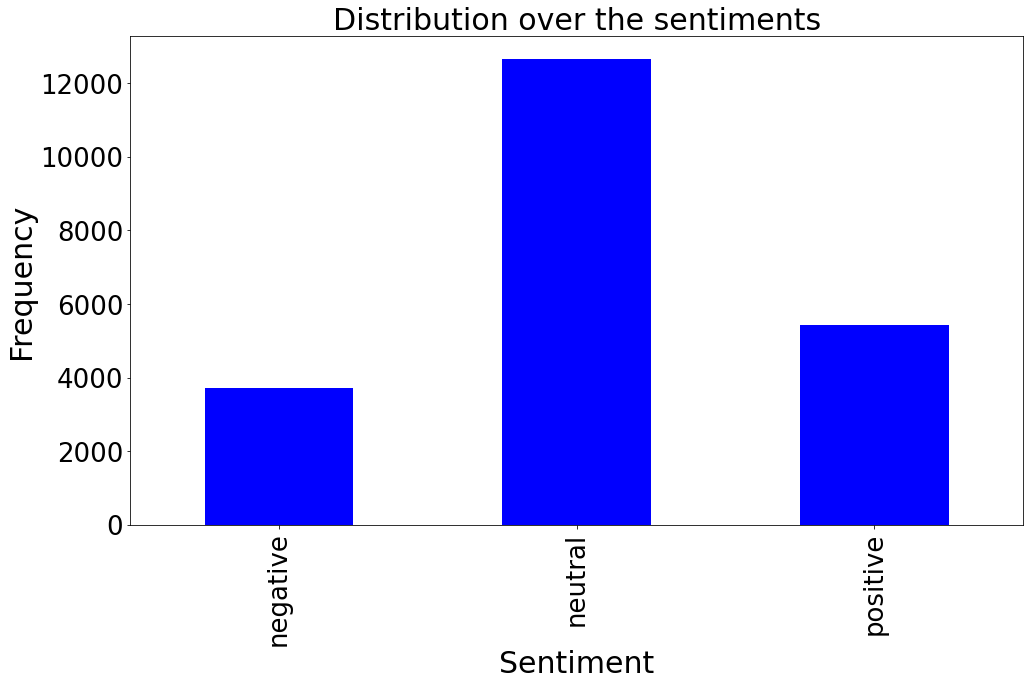
\includegraphics[width = 0.42\textwidth]{sentiment-distribution.png}
	\caption{Distribution of the sentiments}
	\label{fig:sent-dist}
\end{figure} 

\section{Methodology}
% Method: Introduce the used feature(s), and the rationale behind including them. Explain the classifiers
% and evaluation method(s) and metric(s) you have used (and why you have used them). This should be
% at a conceptual level; a detailed description of the code is not appropriate for the report. The description
% should be similar to what you would see in a machine learning conference paper.

This section contains a breakdown of the process through which I develop the final models chosen in Section~\ref{sec:results}.
The following methods are developed with reference to prior works on {T}witter sentiment analysis by Go et al. \shortcite{go09} and Barbosa and Feng \shortcite{robustnoisy10}.

\subsection{Instance Cleaning}

Some of the features extracted rely on the text in the tweets to be pruned of unwanted characters and words.
I have opted to generate a separate list containing the cleaned versions of tweets.
Cleaning involves removing stopwords (Section~\ref{sec:stopwords}), links, tweet hashtags, tweet mentions, numbers, non-alphanumeric characters.
Also performed is the reduction of repeated letters with more than two occurrences to just two, as suggested by Go et al. \shortcite{go09}.

\subsubsection{Stopwords}\label{sec:stopwords}

Manual stopword list construction is tedious and often inexhaustive (especially if I can only determine English stopwords). 
Therefore, I have opted to start with the {P}ython Natural Language Toolkit's (\texttt{NLTK}) defined stopword list, which includes multiple languages \cite{nltk}.
However, since I do not want to blindly rely on this list, 
I generate a set of word clouds over the training cleaned tweets (using the \texttt{NLTK} stopword list) grouped by sentiment.
This then informs whether I need to manually add a few terms which the used list does not include.

\subsection{Feature Extraction}

\subsubsection{{T}witter Features}

First, relying on personal usage experience with {T}witter, I extract the main platform-specific features from the tweet text.
These are:
\begin{itemize}
	\item \textbf{Hashtags} (e.g. \texttt{\#term}): Used to associate tweets with a certain term on the platform.
	\item \textbf{Mentions} (e.g. \texttt{@user}): Used when addressing a specific user on the platform.
	\item \textbf{Links} (e.g. \texttt{https://t.co/id}): Used to link to a website with an id on the platform's redirect service.
\end{itemize}  

These are integrated within the {T}witter platform, meaning they are widely used by users.
Therefore, these features may be strongly correlated to the sentiments and should be isolated for use in the final models.

\subsubsection{Linguistic Features}

Next, linguistic features are extracted and used to tokenize the tweet in different ways. 

\begin{itemize}
	\item \textbf{Part-of-Speech Tags}: Extracting the grammar types of words.
	\item \textbf{Words}: Words used in the tweet.
	\item \textbf{Word 2-Grams}: Word pairs used in the tweet.
	\item 
\end{itemize}  

These feature types may all have certain features which are strongly correlated to a certain sentiment.
For example, a positive \texttt{big win} versus a negative \texttt{big disaster} word pairing.

Neither stemming nor lemmatization are used in the final models as both are too language-dependent.
An example for this is the stemming of \texttt{bare} to \texttt{bar}, removing meaning from the word.
The best option, a multilinguistic lemmatizer, requires a neural network and training \cite{lemmat19}.

\begin{itemize}
	\item \textbf{Punctuation} (\texttt{.?!,:;-()[]\{\}"'/}): Certain punctuation such as exclamation marks may indicate a non-neutral tweet, for example.
	\item \textbf{Emoticons} (e.g. \texttt{:(} or \texttt{:)}): The rise of \texttt{ASCII} emoticons allows users to quickly express their emotions, which correlate strongly to the sentiment of their text.
\end{itemize}  

Extracting emoticons is done differently to the method used in the Go et al. \shortcite{go09} research,
since there are emoticons which are not considered, such as the backwards happy \texttt{(:} emoticon or the cutesie \texttt{:3}.
Instead, emoticons are defined as a string comprised of eye characters (\texttt{;:8=}), optional middle characters (\texttt{,'-"*}), 
and mouth characters divided into four categories: happy (\texttt{)3]}), sad (\texttt{\\/([}), neutral (\texttt{pl|}) and surprised (\texttt{vo}).
There are also defined backwards versions of the happy and sad mouths.
On top of the basic emoticons, others that can be detected are: \texttt{;3}, \texttt{:'o} or \texttt{]":}. 
The detected emoticons are then simplified into one of four emoticons based on their mouth's category: happy \texttt{:)}, sad \texttt{:(}, neutral \texttt{:|} and surprised \texttt{:o}.

\begin{itemize}
	\item \textbf{}
\end{itemize}

\subsubsection{Metric Features}

These are largely numeric counts of other features in a tweet.

\begin{itemize}
	\item \textbf{Number of Words}: More words could indicate a more sentimental tweet.
	\item \textbf{Number of Characters}: It may be that longer tweets contain more non-neutral sentiments than shorter ones.
	\item \textbf{Number of Alphabetic Characters}: This will be correlated to more writing, which has a higher chance of being sentimental.
	\item \textbf{Number of Links}: More linking could indicate a less sentimental tweet.
	\item \textbf{Number of Hashtags}: More hashtags could indicate a more sentimental tweet.
	\item \textbf{Number of Mentions}: More mentions could indicate a more sentimental tweet.
	\item \textbf{Number of Emoticons}: More emoticons could indicate a more sentimental tweet.
	\item \textbf{Retweets} (e.g. \texttt {"text"}): Whether a post quotes another post on the platform. This form of quoting could be used for argumentation.
	\item \textbf{Average Word Length}: Tweets with longer words may tend in a certain direction.
\end{itemize}

\subsubsection{Vectorization}

For all features except the metric features, they can be vectorized by TF-IDF, or occurrence counts.
At the time that the data was collected, tweets were limited to 140 characters \cite{tweetlen}.
This suggests that most features (such as word pairs) are not likely to appear the same time more than once in a tweet (except for stopwords).
Therefore, most features are vectorized with raw counts. 
Certain features that may appear more than once per tweet have their vectorization method chosen using the bar-graph comparison test described in Section~\ref{sec:bargraphs}.

\subsection{Feature Selection}

There are many candidates for features to analyse the sentiments of the tweets.
Using all of them may result in overfitting of the models and increases the time and space complexity of model construction.
To avoid these issues, a certain subset of the features is selected using the following tests.

\subsubsection{Bar Graph Comparison Test}\label{sec:bargraphs}

One way I use to determine the predictive potential of a feature is through comparitive bar graphs.
I generate bar graphs comparing the distributions over the top 10 features in a feature set by the averages of their values, such that:
\begin{equation*}
	\emph{average}_{\sigma \subset S} = \frac{\sum f_{\sigma \subset S}}{\sum f_S}
\end{equation*}
where $\sigma$ is a subset of all the sentiments $S$, $f$ is the vector of values per tweet for a specific feature in a feature type.
If too many of the same features appear in all sentiments' bar graphs, then the feature type is removed from the final feature list.

\subsubsection{Max Features Number}

In a set with $20000+$ instances, the number of possible linguistic features is quite high.
Therefore, I chose to perform a test with the chosen feature types by taking 

% \section{Old Methodology}

% \subsection{Raw Data Analysis}
% First, the dataset was looked at based on the raw data as it came.
% The raw tweets are strings of lowercase text and contain misspelled words, non-alphanumeric characters, Twitter-specific features (mentions and hashtags), and foreign language.

% The distribution of the sentiment labels across the training set was also considered, 
% displaying a clear majority of neutral tweets \ref{fig:sent-dist}.

% \subsection{Preprocessing}

% \subsubsection{Cleaning}
% Some features required the text instances be cleaned before extraction.
% Cleaning involves pruning the tweet of certain characters and features to varying degrees.
% Usually, this means isolating only the alphabetic characters in the text, and performing simple casefolding.
% Since all instances in the dataset are lowercase, only removal of unwanted characters was necessary.
% A type of cleaning considered was the removal of repeated consecutive characters.
% An example where this may have been useful is when encountering words such as \texttt{hey}, which can also appear as \texttt{heyyy}.
% One issue with this method of avoiding suffixing is that it can change the meanings of certain words. For example, \texttt{good} becomes \texttt{god}.
% Extreme suffixing can also be circumvented through stemming or lemmatization, which are discussed in Sections~\ref{sec:stems} and \ref{sec:lemmas}.

% % However, consecutive repeated character pruning was arguably just a primitive, 
% % but language-agnostic implementation of stemming or lemmatization, which are discussed in Section~\ref{subsection:tokens}.
% % Determining the best 

% \subsubsection{Stems}\label{sec:stems}
% Using the Porter stemmer algorithm, the roots of words can be found by removing common English stems. 
% This was considered as an alternative to tokenising by words. 
% However, this may be less effective with words that aren't in English (as they may use different suffixes).
% This method is tested ...

% \subsubsection{Lemmas}\label{sec:lemmas}
% Lemmatization finds the true root of words based on their language definitions.
% Implementing lemmatization required a vast corpus of different languages, 
% with the possibility of overlapping lemmas. 
% The corpus recommended in \texttt{NLTK} contains only the English language. 
% Therefore it was not used to generate results.
% This suffers from the same drawback as stemming, relying the text being in English.

% \subsubsection{Stopwords}

% Initially, the dataset was analyzed to see how different words are distributed throughout it.
% This yielded a word cloud over both the training and testing sets, with the most common words being considered for the stopword list (Figure~\ref{fig:wc-all}).

% \begin{figure}[!h]
% 	\centering
% 	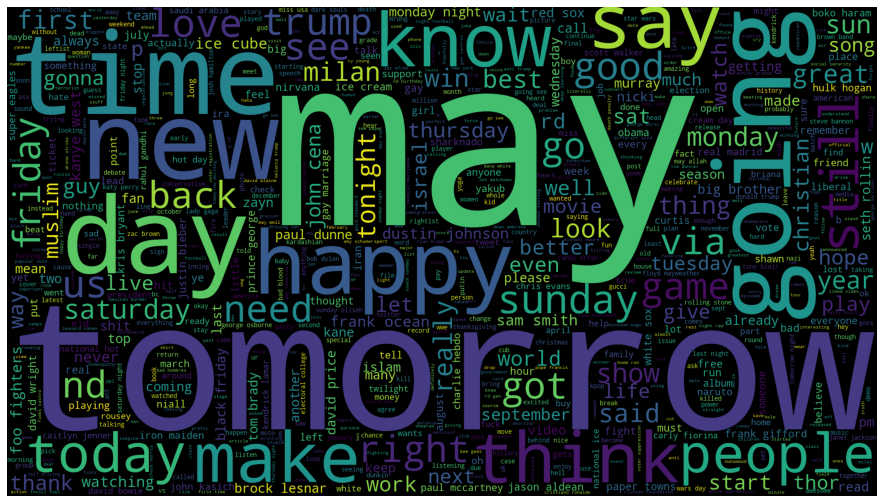
\includegraphics[width = 0.45\textwidth]{wc/all-clean-final.png}
% 	\caption{Word cloud over all tweets}
% 	\label{fig:wc-all}
% \end{figure} 

% The construction of the list was contextual, as some words that appear frequently may still be useful for sentiment analysis.
% To get a better picture of these common, but useful words, three more word clouds were constructed over the word lists per sentiment (Figures~\ref{fig:wc-pos}, \ref{fig:wc-neu}, and \ref{fig:wc-neg}).

% \begin{figure}[!h]
% 	\centering
% 	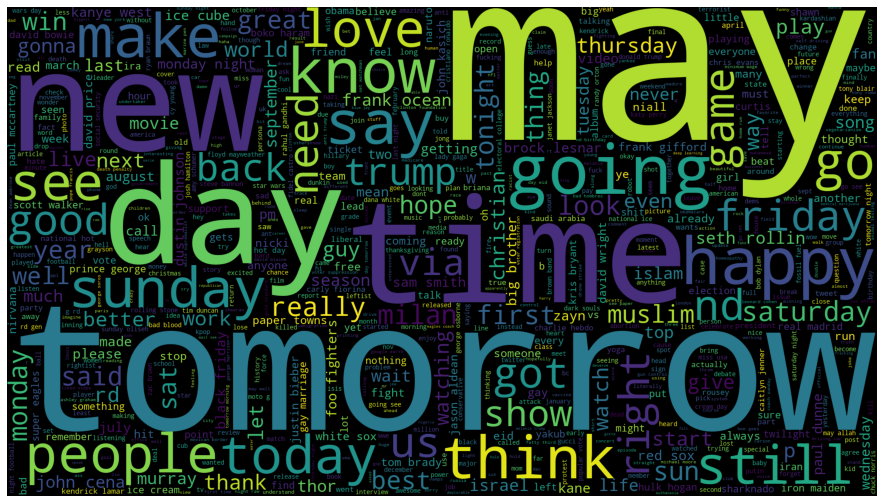
\includegraphics[width = 0.45\textwidth]{wc/positive-clean-final.png}
% 	\caption{Word cloud over positive training tweets}
% 	\label{fig:wc-pos}
% \end{figure} 

% \begin{figure}[!h]
% 	\centering
% 	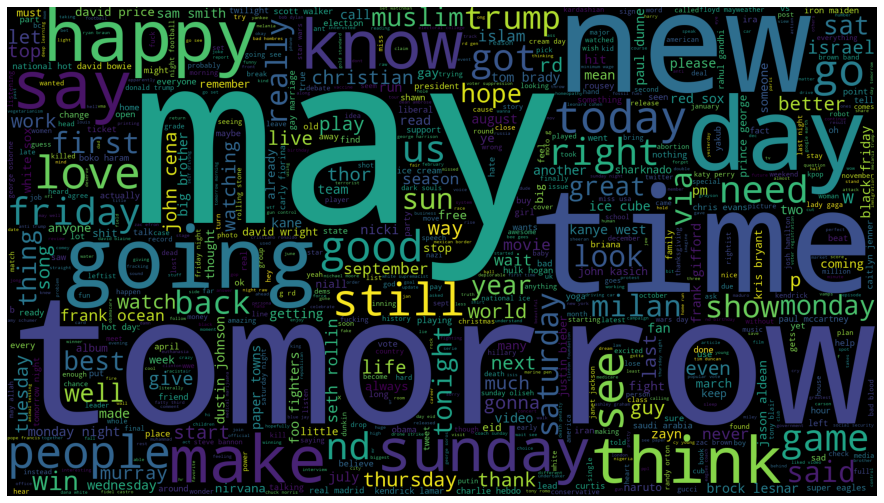
\includegraphics[width = 0.45\textwidth]{wc/neutral-clean-final.png}
% 	\caption{Word cloud over neutral training tweets}
% 	\label{fig:wc-neu}
% \end{figure} 

% \begin{figure}[!h]
% 	\centering
% 	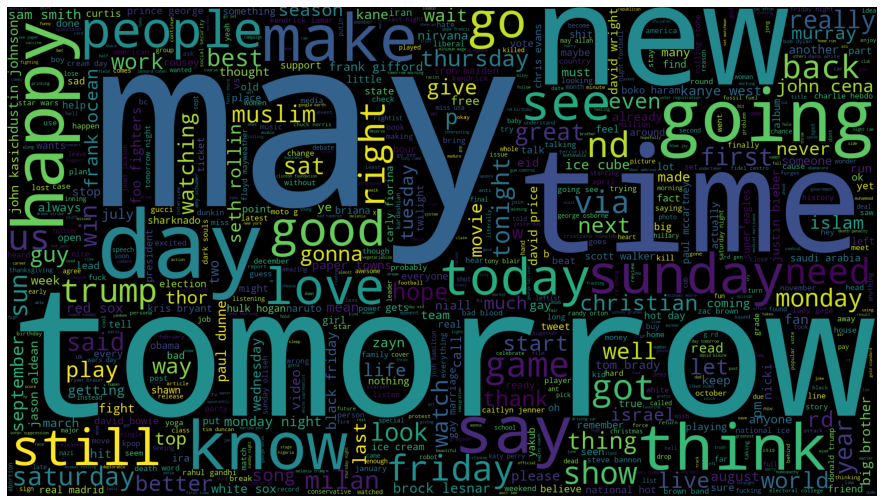
\includegraphics[width = 0.45\textwidth]{wc/negative-clean-final.png}
% 	\caption{Word cloud over negative training tweets}
% 	\label{fig:wc-neg}
% \end{figure} 

% However this method did not consider stopwords in other languages (since English tweets are an overwhelming majority in the dataset).
% Since manual stopword list construction was not as exhaustive as the data required,
% the {P}ython \texttt{NLTK} module's stopword corpus is used where necessary \cite{nltk}.

% \subsection{Vectorization}

% Classifiers in the \texttt{SciKit-learn} {P}ython library require that all data be vectorized to a real-valued space.
% The following vectorizers were used.

% \subsubsection{Count}

% Vectorising the tweet into term counts can highlight terms which appear more often in tweets for certain sentiments.
% This is implemented using \texttt{SciKit-learn}'s \texttt{CountVectorizer} \cite{skl}.

% \subsubsection{TF-IDF}

% This measure of relative word frequency provides more insight, 
% as it measures words that appeach more often in one tweet relative to their overall frequency.
% This is implemented using \texttt{SciKit-learn}'s \texttt{TfidfVectorizer} \cite{skl}.

% \subsubsection{Metrics}

% The final type of vectorization that will occur is in the form of metrics. 
% Certain metrics such as world length may be distributed differently based on the sentiment of the tweet.
% This is implemented by creating a list of mappings to metrics, then vectorizing with \texttt{SciKit-learn}'s \texttt{DictVectorizer} \cite{skl}.

% \subsubsection{Why not hashing?}

% The \texttt{SciKit-learn} library suggests another text feature extractor in the form of hashing.
% This is not used here as the distinct advantage this vectorizer has over others is saving on space and time \cite{skl}.
% While the dataset contains more than 20000 tweets, using the other vectorizers did not present such issues in practice.

% \subsection{Features}\label{subsection:tokens}

% While the data is given as a raw text format, there are multiple features which can be extracted for the purpose of sentiment analysis.

% \subsubsection{N-grams}

% This includes extraction of individual words or characters (1-grams of each) and word pairings (2-grams).
% If $N > 1$, important orderings/configurations of words can be identified, but at the cost of exponentially increasing the possible number of features.
% With a vocabulary of $w$ unique words, there can be as many as $w^N$ distinct N-grams.
% Therefore, the N-grams used for model construction were 1-grams on words, 1-grams on characters, and 2-grams on words.
% 2-grams on characters were not considered 

% This method will requires that tweets are cleaned, but may not need stopword removal.

% \subsubsection{Word Lengths}

% A tokenization where the tokens generated are the lengths of the words in the tweet.

% \subsubsection{Character Frequencies}

% \subsubsection{Links}

% \subsubsection{Hashtags}

% \subsubsection{Mentions}

% \subsubsection{Emoticons}

% \subsubsection{Simple Metrics}

% \subsubsection{Phonetic Frequencies}

% \subsubsection{Poetic Phonetics}

% \subsection{Model Selection}

% \subsubsection{Feature Selection}

% \subsubsection{Classifiers}

% \subsubsection{Evaluation Metrics}

% \section{Results}\label{sec:results}
% % Results: Present the results, in terms of evaluation metric(s) and, ideally, illustrative examples and diagrams.

% \subsection{aw data}

\section{Analysis}
% Discussion / Critical Analysis: Contextualise the systems' behaviour, based on the understanding of the
% subject materials (This is the most important part of the task in this assignment).

% Contextualise implies that we are more interested in seeing evidence of you have thought about the task
% and determining reasons for the relative performance of different methods, rather than the raw scores of
% the different methods you selected. This is not to say that you should ignore the relative performance of
% different runs over the data, but rather that you should think beyond simple numbers to the reasons that
% underlie them.

\section{Conclusions}
% Conclusion: Demonstrate your identified knowledge about the problem.

\bibliographystyle{acl}
\bibliography{citations}

\end{document}
